%!TEX root = ../slides.tex

\section{Виртуальные ПЭТ-изображения}


\begin{frame}
    \frametitle{Виртуальные ПЭТ-изображения}
    Несмотря на то, что ПЭТ-исследование имеет большое количество положительных сторон, у него имеются противопоказания и метод остается труднодоступным для некоторых категорий людей:
    \begin{itemize}
        \item радиоактивный компонент опасен для определенной категории пациентов даже в малых дозах
        \item метод дорогостоящий
        \item ПЭТ - аппараты имеются не во всех медицинских центрах, отдаленных регионах
    \end{itemize}

\end{frame}

\begin{frame}
    \begin{figure}
        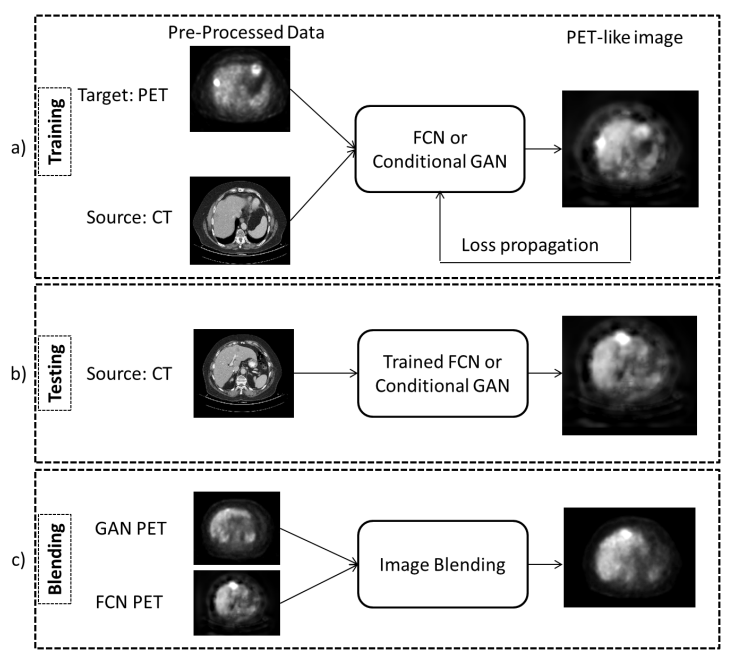
\includegraphics[scale=0.3]{virtual.png}
    \end{figure}
\end{frame}

\begin{frame}
    \begin{figure}
        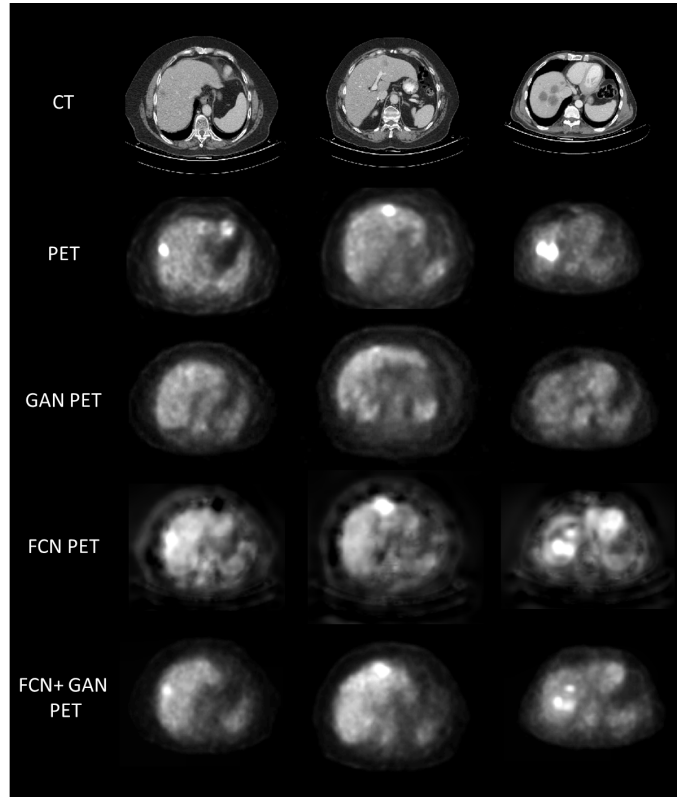
\includegraphics[scale=0.28]{virtualG.png}
    \end{figure}
\end{frame}

